\section{Теории: интуиция}

В этом пункте мы попытаемся на очень неформальном интуитивном уровне понять в чем состоят базовые вопросы логики и откуда они возникают при рассмотрении математических теорий, которые, на первый взгляд, отношения непосредственного к логике не имеют. Это будет очень неформальный материал, и я заранее должен оговориться, что подходы и определения, которые я буду здесь приводить, очень утрированы и упрощены. Абсолютная строгость нам здесь и не нужна, важно понять лишь основы. Формальные определения будут даны в \textsection~1.7, хотя и там мы ограничимся лишь определениями.

Исторически первой математической работой, претендующей на строгое формальное построение математики были <<Начала>> Евклида. После нескольких неформальных определний геометрии на плоскости, Евклид приводил 5 аксиом, которые предлагалось принять без доказательсва, а далее, уже исходя из этих пяти аксиом, выводилиь все теоремы (шесть томов).

Определения были им даны довольно невразумительные. Так, первыми двумя определял точку как <<то, что не имеет никакой части>> и линию как <<длину без ширины>>. Это, вероятно, как-то отражает интуитивные представления, но не даёт ни точного определния, ни свойств. Например, Евклид, ссылаясь в этих определениях на <<части>>, <<длину>> и <<ширину>> сами эти понятия нигде не определяет.

Это на самом деле общая ситуация с любой теорией. Если мы даём какое-то определение, то мы обязаны пользоваться некими понятиями, определенными ранее. При для этих более ранних определений так же должны быть определения. Процесс может продолжаться бесконечно и мы никогда не сможем придти к определению, которое не пользуется никакими другими определниями.

Таким образом, какую бы теорию мы не строили, мы неминуемо приходим к тому, что в самом начале нам необходимо ввести некое понятие, которые мы не определяем никак, просто констатируем как факт, что есть некий объект (неопределенный), которому мы придумываем названия и говорим какие мы с ним можем делать операции и какими свойствами он обладает --- это и есть аксиомы.

Для наших нужд мы пока будем считать, что у нас есть следующие неопределяемые понятия --- \term{точка}, \term{прямая}, \term{перпендикуляр}. Этот список сильно избыточен, что чтобы не углубляться в скучные детали, мы остановимся на этом (далее мы сформулируем аксиомы, которые отчасти определят эти понятия). Будем, однако, считать, что прямая состоит из точек. \term{Пересечением} прямых будем называть точку, которая принадлежит обоим прямым.

\term{Отрезком} мы будем называть две различные точки. Это не совсем корректно, конечно, но нам пока хватит. Если эти точки обозначать как $a$ и $b$, то отрезок мы будем обозначать как $ab$. Мы будем говорить, что две прямые \term{параллельны}, если они не пересекаются (это в точности геометрическое определние для плоскости). \term{Треугольником} мы будем называть три отрезка, если найдутся такие три различные точки $a$, $b$ и $c$, что они попарно будут являются концами этого отрезка. Сам такой треугольник мы будем обозначать как $abc$, а отрезки, построенные на этих точках, как его стороны. Если все три стороны треугольника равны, мы будем говорить, что треугольник \term{равносторонний}. Само понятие \term{равенства} мы пока тоже примем без определения.

\term{Окружностью} мы будем называть объект, состоящий из точек, для которого найдется такая точка $o$ (самой окружности не принадлежащая, мы будем называеть ее \term{центром} окружности), что для любых точек $a$ и $b$ окружности отрезки $ao$ и $bo$ равны. Любой отрезок, им равный, мы будем называть \term{радиусом} окружности.

Далее Евклид приводит 15 аксиом, но с современной точки зрения их можно резюмировать всего пятью следующими простыми утверждениями (остальные аксиомы оказались избыточны):

\begin{enumerate}
\item Пусть $a$ и $b$ --- две различные точки. Тогда через них можно провести единственную прямую $L$.
\item Пусть $a$ --- точка, не лежащая на прямой $L$. Тогда из $a$ в $L$ можно опустить единственный перпендикуляр.
\item Пусть $a$ --- точка, лежащая на прямой $L$, а $M$ --- некоторый отрезок. Тогда на прямой $L$ можно построить различные точки $b$ и $c$, лежащие от $a$ на расстоянии, равном $M$.
\item Пусть $a$ --- точка и $M$ --- отрезок. Можно построить единственную окружность с центром $a$ и адиусом, равным $M$.
\item Пусть $L$ --- прямая, и $a$ --- точка, на ней не лежащая. Тогда можно простроить единственную прямую $M$, которая будет проходить через $a$ и будет параллельна $L$.
\end{enumerate}

Потом в <<Началах>> следует первая теорема: для любого отрезка с концами $ab$ возможно построить равносторонний треугольник $abc$.

Доказательство строится таким образом (см. русинок 1.1 для наглядной интерпретации): проведем окружность c цетром $a$ и радиусом $ab$, затем окружность того же радиуса, но с центром $b$. Пусть $c$ --- их точка пересечения. Поскольку обе окружности имеют один радиус $ab$, то точка $c$ отстоит от обоих точек $a$ и $b$ на одно и то же расстояние, равное отрезку $ab$. Стало быть точки $a$, $b$ и $c$ образуют равносторонний треугольник.

\begin{figure}[h]
\centering
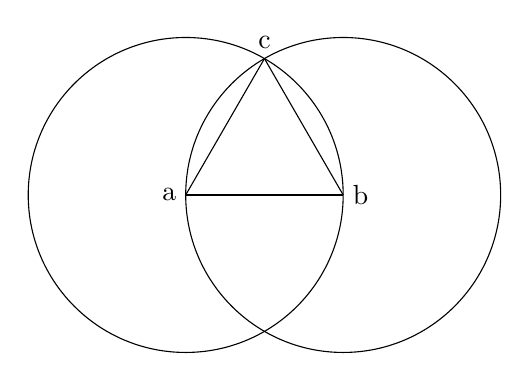
\begin{tikzpicture}
    \draw (-1,0) circle (2) node [anchor=east] {a};
	\draw (1,0) circle (2);
	\draw (-1,0) -- (1,0) node [anchor=west] {b};
	\draw (-1,0) -- (0,1.7321) node [anchor=south] {c};
	\draw (0,1.7321) -- (1,0);
\end{tikzpicture}
\caption{Построение равностороннего треугольника}
\end{figure}

Вроде бы вполне себе наглядное и очевидное доказательство, какие к нему могут быть вопросы? На самом деле это доказательство некорректно, но прежде чем мы сформулируем наши к нему претензии, переведем всё сказанное на язык логики.

Вначале переформулируем аксиомы. С точки зрения логики, у нас нет никакой разницы между различными объектами --- все символы, какими мы пользуемся, едины. Чтобы их различать, нам необходимо ввести предикаты. Например, пусть предикат $P$ обозначает свойство <<быть точкой>>, а предикат $Q$ <<быть прямой>>. Тогда первая аксиома может быть записана как $$\forall a \forall b (a\not=b \land P(a) \land P(b) \to \exists L (Q(L) \land a \in L \land b \in L))$$

Довольно неприятная формула. 